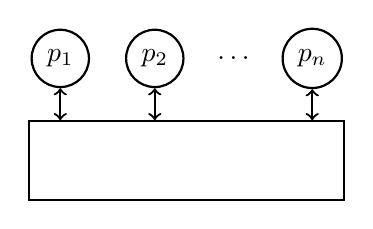
\begin{tikzpicture}
\node[circle, thick, draw] (v1) at (-0.2,0.8) {$p_1$};
\node[circle, thick, draw] (v3) at (1,0.8) {$p_2$};
\node at (2,0.8) {$\dots$};
\node[circle, thick, draw] (v5) at (3,0.8) {$p_n$};

\node (v2) at (-0.2,-0.11) {};
\node (v4) at (1,-0.11) {};
\node (v6) at (3,-0.11) {};

\draw[thick] (-0.6,0) rectangle (3.4,-1);

\draw[<->, thick]  (v1) edge (v2);
\draw[<->, thick]  (v3) edge (v4);
\draw[<->, thick]  (v5) edge (v6);

\end{tikzpicture}